% Options for packages loaded elsewhere
\PassOptionsToPackage{unicode}{hyperref}
\PassOptionsToPackage{hyphens}{url}
%
\documentclass[
]{article}
\usepackage{amsmath,amssymb}
\usepackage{lmodern}
\usepackage{ifxetex,ifluatex}
\ifnum 0\ifxetex 1\fi\ifluatex 1\fi=0 % if pdftex
  \usepackage[T1]{fontenc}
  \usepackage[utf8]{inputenc}
  \usepackage{textcomp} % provide euro and other symbols
\else % if luatex or xetex
  \usepackage{unicode-math}
  \defaultfontfeatures{Scale=MatchLowercase}
  \defaultfontfeatures[\rmfamily]{Ligatures=TeX,Scale=1}
\fi
% Use upquote if available, for straight quotes in verbatim environments
\IfFileExists{upquote.sty}{\usepackage{upquote}}{}
\IfFileExists{microtype.sty}{% use microtype if available
  \usepackage[]{microtype}
  \UseMicrotypeSet[protrusion]{basicmath} % disable protrusion for tt fonts
}{}
\makeatletter
\@ifundefined{KOMAClassName}{% if non-KOMA class
  \IfFileExists{parskip.sty}{%
    \usepackage{parskip}
  }{% else
    \setlength{\parindent}{0pt}
    \setlength{\parskip}{6pt plus 2pt minus 1pt}}
}{% if KOMA class
  \KOMAoptions{parskip=half}}
\makeatother
\usepackage{xcolor}
\IfFileExists{xurl.sty}{\usepackage{xurl}}{} % add URL line breaks if available
\IfFileExists{bookmark.sty}{\usepackage{bookmark}}{\usepackage{hyperref}}
\hypersetup{
  pdftitle={CR TP1 Programmation par contraintes},
  pdfauthor={Julien LETOILE, Romain HUBERT},
  hidelinks,
  pdfcreator={LaTeX via pandoc}}
\urlstyle{same} % disable monospaced font for URLs
\usepackage{graphicx}
\makeatletter
\def\maxwidth{\ifdim\Gin@nat@width>\linewidth\linewidth\else\Gin@nat@width\fi}
\def\maxheight{\ifdim\Gin@nat@height>\textheight\textheight\else\Gin@nat@height\fi}
\makeatother
% Scale images if necessary, so that they will not overflow the page
% margins by default, and it is still possible to overwrite the defaults
% using explicit options in \includegraphics[width, height, ...]{}
\setkeys{Gin}{width=\maxwidth,height=\maxheight,keepaspectratio}
% Set default figure placement to htbp
\makeatletter
\def\fps@figure{htbp}
\makeatother
\setlength{\emergencystretch}{3em} % prevent overfull lines
\providecommand{\tightlist}{%
  \setlength{\itemsep}{0pt}\setlength{\parskip}{0pt}}
\setcounter{secnumdepth}{-\maxdimen} % remove section numbering
\ifluatex
  \usepackage{selnolig}  % disable illegal ligatures
\fi

\title{CR TP1 Programmation par contraintes}
\author{Julien LETOILE, Romain HUBERT}
\date{}

\begin{document}
\maketitle

\hypertarget{header-n3}{%
\section{\texorpdfstring{CR TP1 Programmation par contraintes
}{CR TP1 Programmation par contraintes }}\label{header-n3}}

Julien LETOILE, Romain HUBERT

le 26/01/2021

\hypertarget{header-n16}{%
\subsection{Table des matières}\label{header-n16}}

\begin{center}\rule{0.5\linewidth}{0.5pt}\end{center}

\tableofcontents

\begin{center}\rule{0.5\linewidth}{0.5pt}\end{center}

\hypertarget{header-n21}{%
\subsection{\texorpdfstring{I. \underline{Réponses
rédigées}}{I. Réponses rédigées}}\label{header-n21}}

\hypertarget{header-n22}{%
\subsubsection{Question 1.2}\label{header-n22}}

Prolog permet de tester automatiquement les contraintes sur toutes les
données en les unifiant sous la forme d'arbres. Cela en fait un solveur
de contraintes sur le domaine des arbres.

\hypertarget{header-n24}{%
\subsubsection{Question 1.6}\label{header-n24}}

Prolog ne comprend pas les signes mathématiques, mais est capable de
calculer de manière très efficace.\\
Si l'on pose le prédicat \emph{\textgreater=} avant les appels à
\emph{isBetween}, on obtient un \emph{instanciation fault}.\\
On parle d'approche "Generate and Test" puisque dans \emph{commande}, on
va d'abord générer les valeurs possibles avec les \emph{isBetween}, puis
on teste les valeurs générés avec l'inégalité.

\hypertarget{header-n26}{%
\subsubsection{Question 1.7}\label{header-n26}}

En remplaçant les prédicats \emph{isBetween} et \emph{\textgreater=} par
les conraintes \emph{Var \#:: Min..Max} et \emph{\#\textgreater=}, on
obtient la réponse suivante :

\begin{quote}
isBetween2(X, -2, 5).

X = X\{-2 .. 5\}\\
Yes (0.00s cpu)
\end{quote}

\emph{\{-2 .. 5\}} correspond à l'intervalle des valeurs possibles de X
répondant à la contrainte.

\hypertarget{header-n32}{%
\subsubsection{Question 1.12}\label{header-n32}}

Après exécution de la requête \textbf{\emph{X \#:: -10..10, vabs(X,
Y).}}, on obtient la réponse suivante :

\begin{quote}
X = 0\\
Y = 0\\
Yes (0.00s cpu, solution 1, maybe more) ? ;

X = 1\\
Y = 1\\
Yes (0.00s cpu, solution 2, maybe more) ? ;

X = 2\\
Y = 2\\
Yes (0.00s cpu, solution 3, maybe more) ? ;

...

X = -9\\
Y = 9\\
Yes (0.02s cpu, solution 20, maybe more) ? ;

X = -10\\
Y = 10\\
Yes (0.02s cpu, solution 21)
\end{quote}

Après exécution de la requête \textbf{\emph{X \#:: -10..10, vabsOr(X,
Y).}}, on obtient la réponse suivante :

\begin{quote}
X = 0\\
Y = 0\\
Yes (0.00s cpu, solution 1, maybe more) ? ;

X = -10\\
Y = 10\\
Yes (0.00s cpu, solution 2, maybe more) ? ;

X = -9\\
Y = 9\\
Yes (0.00s cpu, solution 3, maybe more) ? ;

...

X = 9\\
Y = 9\\
Yes (0.00s cpu, solution 20, maybe more) ? ;

X = 10\\
Y = 10\\
Yes (0.00s cpu, solution 21)
\end{quote}

On remarque que les 2 sorties se ressemblent hormis une inversion des
arrivées des valeurs de X. Prolog, dans \emph{vabs}, cherche toutes les
solutions de \textbf{\emph{AbsVal \#= Val}} puis les solutions de
\textbf{\emph{AbsVal \#= -Val}}. Alors que dans \emph{vabsOr}, le
labeling prend toutes les valeurs dans l'ordre.

\hypertarget{header-n50}{%
\subsubsection{Question 1.15}\label{header-n50}}

Pour vérifier que cette suite est périodique de période 9, il suffit de
montrer qu'il n'existe pas une suite qui n'est pas de période 9. Ainsi,
une requête qui vérifie cela est:

\begin{quote}
faitListe(X, 15, -100, 100), suite(X), non\_periodique9(X), labeling(X).

No (0.75 cpu)
\end{quote}

Donc la suite est de période 9.

\hypertarget{header-n56}{%
\subsection{\texorpdfstring{II. \underline{Arbres de
recherche}}{II. Arbres de recherche}}\label{header-n56}}

\hypertarget{header-n57}{%
\subsubsection{Question 1.5}\label{header-n57}}

Après exécution de la requête \textbf{\emph{commande(NbResistance,
NbCondensateur).}}, on obtient l'arbre élagué suivant :

\begin{figure}
\hypertarget{mermaid}{%
\centering

\includegraphics[width=4.16667in,height=\textheight]{1611931517726.png}
\caption{}\label{mermaid}
}
\end{figure}

\begin{figure}
\hypertarget{mermaid}{%
\centering

\includegraphics[width=0.29167in,height=\textheight]{1611931517726.png}
\caption{}\label{mermaid}
}
\end{figure}

\hypertarget{header-n66}{%
\subsubsection{Question 1.8}\label{header-n66}}

\begin{figure}
\hypertarget{flow}{%
\centering
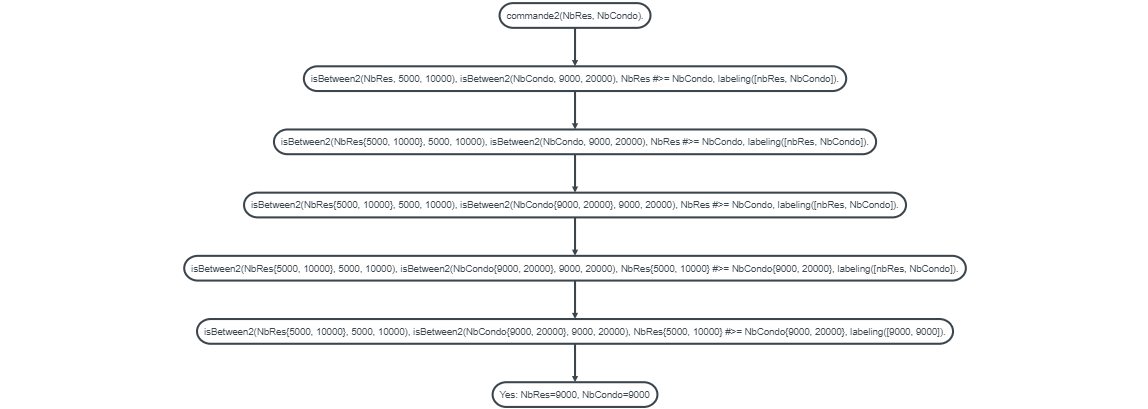
\includegraphics[width=8.20833in,height=\textheight]{1611931517727.png}
\caption{}\label{flow}
}
\end{figure}

\end{document}
